\begin{figure}
   \def\dash{-\phantom{00}}
\begin{small}
\begin{tabular}{@{}l|r:rr|r:rr|r}
Method                                                   & C100  & C100+ & C100++ & C10   & C10+  & C10++ & SVHN \\
\toprule
Network in Network~\citep{nin}                           & 35.68 & \dash & \dash  & 10.41 & 8.81  & \dash & 2.35 \\
Generalized Pooling~\citep{lee2016generalizing}          & 32.37 & \dash & \dash  & 7.62  & 6.05  & \dash & 1.69 \\ % Aug: a bunch of stuff: hue, scaling, etc.
Recurrent CNN~\citep{liang2015recurrent}                 & 31.75 & \dash & \dash  & 8.69  & 7.09  & \dash & 1.77 \\ % Aug: "translations and horizontal (sic) reflections"
Multi-scale~\citep{liao2015competitive}                  & 27.56 & \dash & \dash  & 6.87  & \dash & \dash & 1.76 \\
FitNet~\cite{romero2014fitnets}                          & \dash & 35.04 & \dash  & \dash & 8.39  & \dash & 2.42 \\ % Aug: Uses only flipping, no translation!
Deeply Supervised~\citep{lee2014deeply}                  & \dash & 34.57 & \dash  & 9.69  & 7.97  & \dash & 1.92 \\
All-CNN~\citep{springenberg2014striving}                 & \dash & 33.71 & \dash  & 9.08  & 7.25  & 4.41  & \dash\\ % Aug: mirroring and shifts {-5, ..., 5}, whitening
Highway Net~\citep{srivastava2015highway}                & \dash & 32.39 & \dash  & \dash & 7.72  & \dash & \dash\\ % Aug: Just says "random translations"
ELU~\citep{elu}                                          & \dash & 24.28 & \dash  & \dash & 6.55  & \dash & \dash\\ % Aug: Standard
Scalable BO~\citep{snoek2015scalable}                    & \dash & \dash & 27.04  & \dash & \dash & 6.37  & 1.77 \\ % Aug: a bunch of stuff: hue, scaling, etc.
Fractional Max-Pool~\citep{graham2014fractional}         & \dash & \dash & 26.32  & \dash & \dash & 3.47  & \dash\\ % Aug: built-in
\midrule
FitResNet~\citep{mishkin2015all}                         & \dash & 27.66 & \dash  & \dash & 5.84  & \dash & \dash\\ % Aug: mirroring and shifts
{\Resnet}~\citep{he2015deep}                             & \dash & \dash & \dash  & \dash & 6.61  & \dash & \dash\\ % Aug: mirroring and shifts {-4, ..., 4}
{\Resnet} by~\citep{huang2016stochasticdepth}            & 44.76 & 27.22 & \dash  & 13.63 & 6.41  & \dash & 2.01 \\ % Aug:
Stochastic Depth~\citep{huang2016stochasticdepth}        & 37.80 & 24.58 & \dash  & 11.66 & 5.23  & \dash & 1.75 \\
Identity Mapping~\citep{he2016identity}                  & \dash & 22.68 & \dash  & \dash & 4.69  & \dash & \dash\\
{\Resnet} in {\Resnet}~\citep{rir}                       & \dash & 22.90 & \dash  & \dash & 5.01  & \dash & \dash\\    %  v might swap f195 for f221
Wide~\citep{wideresnet}                                  & \dash & 20.50 & \dash  & \dash & 4.17  & \dash & \dash\\ % They have SVHN too! Not sure which number to report. Need to double-check the CIFAR numbers too, since they report many different numbers.
DenseNet-BC~\citep{densenet}\footnotemark                & 19.64 & 17.60 & \dash  &  5.19 & 3.62  & \dash & 1.74 \\
\midrule
{\Fracnet} (20 layers, 38.6M params)                     & 35.34 & 23.30 & 22.85  & 10.18 & 5.22  & 5.11  & 2.01 \\ % 100:f200/f199/f201 10:f223/f224/f232 S:f233
~+~\droppath~+~\dropout                                  & 28.20 & 23.73 & 23.36  & 7.33  & 4.60  & 4.59  & 1.87 \\ % 100:f221/f234/f235 10:f226/f236/f237 S:f227
\quad\quad%
\raisebox{0.06cm}{$\drsh$} deepest column alone          & 29.05 & 24.32 & 23.60  & 7.27  & 4.68  & 4.63  & 1.89 \\
{\Fracnet} (40 layers, 22.9M params)\footnotemark        & \dash & 22.49 & 21.49  & \dash & 5.24  & 5.21  & \dash\\ % 100:TODO/f277/f296 10:TODO/f295/f297 S:TODO
\bottomrule
\end{tabular}
\end{small}
% experiments there were updated
% f195 -> f221
% f225 -> f233
% f197 -> f234
%
% parens: results and updated job id is not the same - new results are coming

   \captionof{table}{
      \textbf{CIFAR-100/CIFAR-10/SVHN.}
      We compare test error (\%) with other leading methods, trained with
      either no data augmentation, translation/mirroring (+), or more
      substantial augmentation (++).  Our main point of comparison is
      {\resnet}.  We closely match its benchmark results using data
      augmentation, and outperform it by large margins without data
      augmentation.  Training with {\droppath}, we can extract from
      {\fracnet} single-column (plain) networks that are highly competitive.
      %Note: Fractional Pooling is filed under non-standard data augmentation
      %      as argued by~\cite{mishkin2015all}.  It also uses multiple passes
      %      at test time.
   }
\label{tab:all}
\end{figure}

\addtocounter{footnote}{-1}
\footnotetext{%
   Densely connected networks (DenseNets) are concurrent work, appearing
   subsequent to our original arXiv paper on FractalNet.  A variant of residual
   networks, they swap addition for concatenation in the residual functional
   form.  We report performance of their $250$-layer DenseNet-BC network with
   growth rate $k=24$.
}

\stepcounter{footnote}
\footnotetext{%
   This deeper (4 column) {\fracnet} has fewer parameters.  We vary column
   width: $(128, 64, 32, 16)$ channels across columns initially, doubling each
   block except the last.  A linear projection temporarily widens thinner
   columns before joins.  As in~\cite{SqueezeNet}, we switch to a mix of
   $1 \times 1$ and $3 \times 3$ convolutional filters.
}

The CIFAR, SVHN, and ImageNet datasets serve as testbeds for comparison to
prior work and analysis of {\fracnet}'s internal behavior.  We evaluate
performance on the standard classification task associated with each
dataset.  For CIFAR and SVHN, which consist of $32 \times 32$ images, we set
our fractal network to have $5$ blocks ($B=5$) with $2 \times 2$
non-overlapping max-pooling and subsampling applied after each.  This reduces
the input $32 \times 32$ spatial resolution to $1 \times 1$ over the course of
the entire network.  A softmax prediction layer attaches at the end of the
network.  Unless otherwise noted, we set the number of filter channels within
blocks $1$ through $5$ as $(64, 128, 256, 512, 512)$, mostly matching the
convention of doubling the number of channels after halving spatial resolution.

For ImageNet, we choose a fractal architecture to facilitate direct comparison
with the $34$-layer {\resnet} of~\cite{he2015deep}.  We use the same first and
last layer as {\resnet}-34, but change the middle of the network to consist of
$4$ blocks ($B=4$), each of $8$ layers ($C=4$ columns).  We use a filter
channel progression of $(128, 256, 512, 1024)$ in blocks $1$ through $4$.

\subsection{Training}
\label{sec:training}

For experiments using {\dropout}, we fix drop rate per block at
$(0\%, 10\%, 20\%, 30\%, 40\%)$, similar to~\cite{elu}.  Local {\droppath}
uses $15\%$ drop rate across the entire network.

We run for $400$ epochs on CIFAR, $20$ epochs on SVHN, and $70$ epochs on
ImageNet.  Our learning rate starts at $0.02$ (for ImageNet, $0.001$) and we
train using stochastic gradient descent with batch size $100$ (for ImageNet,
$32$) and momentum $0.9$.  For CIFAR/SVHN, we drop the learning rate by a
factor of $10$ whenever the number of remaining epochs halves.  For ImageNet,
we drop by a factor of $10$ at epochs $50$ and $65$.  We use Xavier
initialization~\citep{glorot2010understanding}.

A widely employed~\citep{nin,elu,srivastava2015highway,he2015deep,
he2016identity,huang2016stochasticdepth,rir} scheme for data augmentation on
CIFAR consists of only horizontal mirroring and translation (uniform offsets
in $[-4,4]$), with images zero-padded where needed after mean subtraction.
We denote results achieved using no more than this degree of augmentation by
appending a ``+'' to the dataset name (\eg~CIFAR-100+).  A ``++'' marks
results reliant on more data augmentation; here exact schemes may vary.  Our
entry in this category is modest and simply changes the zero-padding to
reflect-padding.

\begin{figure}
   \begin{minipage}[b]{0.45\linewidth}
      \vspace{0pt}
      % ImageNet
      \begin{center}
      \begin{tabular}{@{}lrr@{}}
Method            & Top-1 (\%) & Top-5  (\%) \\
\toprule
VGG-16            & 28.07      & 9.33 \\
{\Resnet}-34 C    & 24.19      & 7.40 \\
{\Fracnet}-34     & 24.12      & 7.39 \\
\bottomrule
\end{tabular}

      \end{center}
      \vspace{-0.04\linewidth}
      \captionof{table}{
         \textbf{ImageNet}~(validation set, 10-crop).
      }
      \label{tab:imagenet}
      \vspace{0.03\linewidth}
      % Ultra-deep
      \begin{center}
      \begin{tabular}{@{}lrrr@{}}
  Cols. & Depth  & Params.    &  Error (\%)\\
\toprule
     ~1 &      5 &       0.3M &      37.32 \\   % f209
     ~2 &     10 &       0.8M &      30.71 \\   % f210
     ~3 &     20 &       2.1M &      27.69 \\   % f207
     ~4 &     40 &       4.8M &      27.38 \\   % f211
     ~5 &     80 &      10.2M &      26.46 \\   % f212
     ~6 &    160 &      21.1M &      27.38 \\   % f213
\bottomrule
\end{tabular}

      \end{center}
      \vspace{-0.04\linewidth}
      \captionof{table}{
         \textbf{Ultra-deep fractal networks} (CIFAR-100++).
         Increasing depth greatly improves accuracy until eventual diminishing
         returns.  Contrast with plain networks, which are not trainable if
         made too deep (Table~\ref{tab:individual}).
      }
      \label{tab:columns}
   \end{minipage}
   \hfill
   \begin{minipage}[b]{0.51\linewidth}
      \vspace{0pt}
      \begin{center}
      \begin{tabular}{@{}lrrr@{}}
Model                    & Depth          & Train Loss     & Error (\%)     \\
\toprule
Plain                    & 5              & 0.786          & 36.62          \\
Plain                    & 10             & 0.159          & 32.47          \\
Plain                    & 20             & 0.037          & 31.31          \\
\textbf{Plain}           & \textbf{40}    & \textbf{0.580} & \textbf{38.84} \\
\midrule
Fractal Col \#1          & 5              & 0.677          & 37.23          \\
Fractal Col \#2          & 10             & 0.141          & 32.85          \\
Fractal Col \#3          & 20             & 0.029          & 31.31          \\
\textbf{Fractal Col \#4} & \textbf{40}    & \textbf{0.016} & \textbf{31.75} \\
\midrule
\textbf{Fractal Full}    & \textbf{40}    & \textbf{0.015} & \textbf{27.40} \\
\bottomrule
\end{tabular}
%
% f240:
% loss0: 0.785858      63.38
% loss1: 0.158773      67.53
% loss2: 0.0372975     68.69
% loss3: 0.579952      61.16
%
% f241:
% loss0: 0.676799      62.77
% loss1: 0.141266      67.15
% loss2: 0.0292944     68.69
% loss3: 0.0163973     68.25
%
% full:  0.0148776     72.60

      \end{center}
      \vspace{-0.02\linewidth}
      \captionof{table}{
         \textbf{Fractal structure as a training apparatus} (CIFAR-100++).
         Plain networks perform well if moderately deep, but exhibit worse
         convergence during training if instantiated with great depth.
         However, as a column trained within, and then extracted from, a
         fractal network with mixed {\droppath}, we recover a plain network
         that overcomes such depth limitation (possibly due to a
         student-teacher effect).
      }
      \label{tab:individual}
   \end{minipage}
\end{figure}

\subsection{Results}
\label{sec:evaluation}

Table~\ref{tab:all} compares performance of {\fracnet} on CIFAR and SVHN with
competing methods.  {\Fracnet} (depth $20$) outperforms the original {\resnet}
across the board.  With data augmentation, our CIFAR-100 accuracy is close to
that of the best {\resnet} variants.  With neither augmentation nor
regularization, {\fracnet}'s performance on CIFAR is superior to both {\resnet}
and {\resnet} with stochastic depth, suggesting that {\fracnet} may be less
prone to overfitting.  Most methods perform similarly on SVHN.  Increasing
depth to $40$, while borrowing some parameter reduction tricks~\citep{
SqueezeNet}, reveals {\fracnet}'s performance to be consistent across a range
of configuration choices.

Experiments without data augmentation highlight the power of {\droppath}
regularization.  On CIFAR-100, {\droppath} reduces {\fracnet}'s error rate
from $35.34\%$ to $28.20\%$.  Unregularized {\resnet} is far behind ($44.76\%$)
and {\resnet} with stochastic depth ($37.80\%$) does not catch up to our
unregularized starting point of $35.34\%$.  CIFAR-10 mirrors this story.  With
data augmentation, {\droppath} provides a boost (CIFAR-10), or does not
significantly influence {\fracnet}'s performance (CIFAR-100).

Note that the performance of the deepest column of the fractal network is
close to that of the full network (statistically equivalent on CIFAR-10).
This suggests that the fractal structure may be more important as a
learning framework than as a final model architecture.

Table~\ref{tab:imagenet} shows that {\fracnet} scales to ImageNet,
matching {\resnet}~\citep{he2015deep} at equal depth.  Note that, concurrent
with our work, refinements to the residual network paradigm further improve
the state-of-the-art on ImageNet.  Wide residual networks~\citep{wideresnet}
of $34$-layers reduce single-crop Top-1 and Top-5 validation error by
approximately $2\%$ and $1\%$, respectively, over ResNet-$34$ by doubling
feature channels in each layer.  DenseNets~\citep{densenet} substantially
improve performance by building residual blocks that concatenate rather than
add feature channels.

Table~\ref{tab:columns} demonstrates that {\fracnet} resists performance
degradation as we increase $C$ to obtain extremely deep networks ($160$ layers
for $C=6$).  Scores in this table are not comparable to those in
Table~\ref{tab:all}.  For time and memory efficiency, we reduced block-wise
feature channels to $(16, 32, 64, 128, 128)$ and the batch size to $50$ for the
supporting experiments in Tables~\ref{tab:columns} and~\ref{tab:individual}.

Table~\ref{tab:individual} provides a baseline showing that training of plain
deep networks begins to degrade by the time their depth reaches $40$ layers.
In our experience, a plain $160$-layer completely fails to converge. This
table also highlights the ability to use {\fracnet} and {\droppath} as an
engine for extracting trained networks (columns) with the same topology as
plain networks, but much higher test performance.

\begin{figure}
   \begin{center}
      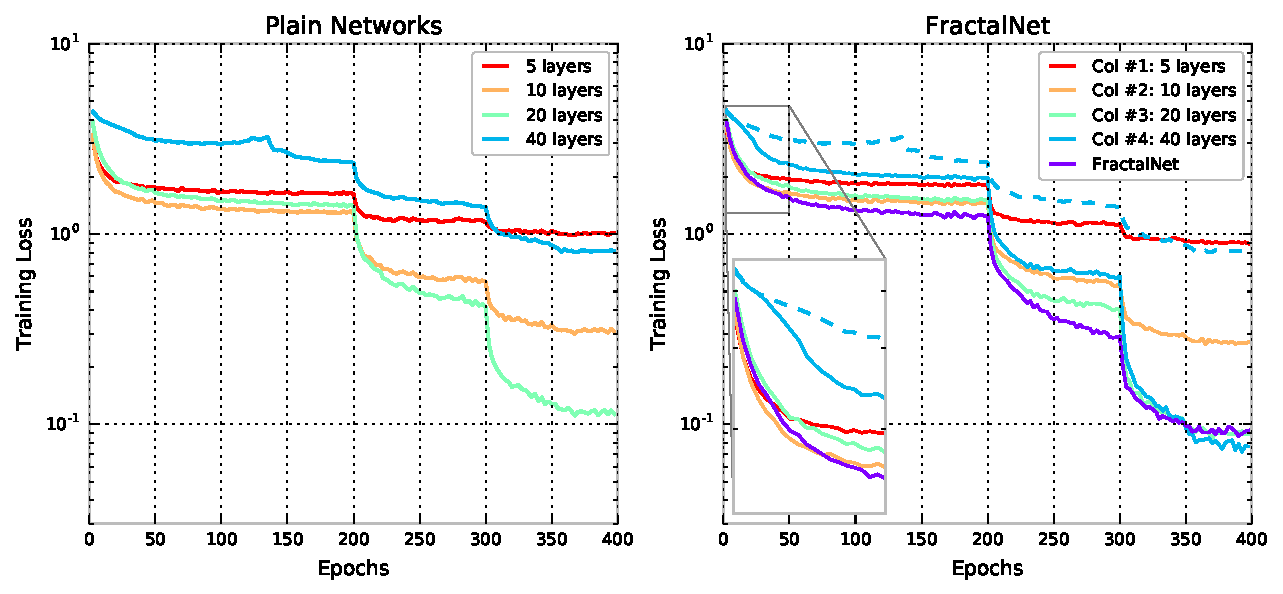
\includegraphics[width=1.0\linewidth]{figures/fractalnet-loss.pdf}
   \end{center}
   \vspace{-0.4cm}
   \caption{
      \textbf{Implicit deep supervision.}
      \emph{Left:}
         Evolution of loss for plain networks of depth $5$, $10$, $20$ and
         $40$ trained on CIFAR-100.  Training becomes increasingly difficult
         for deeper networks.  At $40$ layers, we are unable to train the
         network satisfactorily.
      \emph{Right:}
         We train a $4$ column fractal network with mixed \droppath{},
         monitoring its loss as well as the losses of its four subnetworks
         corresponding to individual columns of the same depth as the plain
         networks.  As the $20$-layer subnetwork starts to stabilize,
         \droppath{} puts pressure on the $40$-layer column to adapt, with the
         rest of the network as its teacher.  This explains the elbow-shaped
         learning curve for Col \#4 that occurs around $25$ epochs.
   }
\label{fig:fractalnet-loss}
\end{figure}

\subsection{Introspection}
\label{sec:introspection}

With Figure~\ref{fig:fractalnet-loss}, we examine the evolution of a $40$-layer
{\fracnet} during training.  Tracking columns individually (recording their
losses when run as stand-alone networks), we observe that the $40$-layer column
initially improves slowly, but picks up once the loss of the rest of the
network begins to stabilize.  Contrast with a plain $40$-layer network trained
alone (dashed blue line), which never makes fast progress.  The column has the
same initial plateau, but subsequently improves after $25$ epochs, producing a
loss curve uncharacteristic of plain networks.

We hypothesize that the fractal structure triggers effects akin to deep
supervision and lateral student-teacher information flow.  Column \#4 joins
with column \#3 every other layer, and in every fourth layer this join
involves no other columns.  Once the fractal network partially relies on the
signal going through column \#3, {\droppath} puts pressure on column \#4 to
produce a replacement signal when column \#3 is dropped.  This task has
constrained scope.  A particular drop only requires two consecutive layers in
column \#4 to substitute for one in column \#3 (a mini student-teacher
problem).

This explanation of FractalNet dynamics parallels what, in concurrent
work, \cite{unrolled} claim for ResNet.  Specifically, \cite{unrolled} suggest
residual networks learn unrolled iterative estimation, with each layer
performing a gradual refinement on its input representation.  The deepest
FractalNet column could behave in the same manner, with the remainder of the
network acting as a scaffold for building smaller refinement steps by doubling
layers from one column to the next.

These interpretations appear not to mesh with the conclusions of~\cite{
veit16residual}, who claim that ensemble-like behavior underlies the success of
ResNet.  This is certainly untrue of some very deep networks, as FractalNet
provides a counterexample: we can extract a single column (plain network
topology) and it alone (no ensembling) performs nearly as well as the entire
network.  Moreover, the gradual refinement view may offer an alternative
explanation for the experiments of~\cite{veit16residual}.  If each layer makes
only a small modification, removing one may look, to the subsequent portion of
the network, like injecting a small amount of input noise.  Perhaps noise
tolerance explains the gradual performance degradation that \cite{
veit16residual} observe when removing ResNet layers.
